\documentclass{article}

\usepackage[francais]{babel}
\usepackage[T1]{fontenc}
\usepackage{geometry}
\geometry{hmargin=2.5cm}
\usepackage{amsmath}
\usepackage{graphicx}
\usepackage{subcaption}
\usepackage{float}
\usepackage{hyperref}
\usepackage{setspace}
\usepackage{xcolor}
\usepackage{pdfpages}
\usepackage{enumitem}
\usepackage{lscape}

\title{Jeu awélé\bigbreak \bigbreak
    \large Analyse UML}

\date{20 mai 2020}
\author{Laura Binacchi}

\begin{document}
    \pagenumbering{gobble}
    
\includepdf[pages={1}]{pdg}
    \newpage
    \tableofcontents
    \newpage
    \pagenumbering{arabic}

    \section*{Introduction}
    \label{sec:intro}
    \addcontentsline{toc}{section}{\nameref{sec:intro}}

    \paragraph{}
    %Ce travail présente l'analyse UML du jeu awélé réalisée dans le cadre du cours de Programmation orientée objet. L'awélé est un jeu de semailles d'origine africaine dont le but est de récolter le maximum de graines sur un plateau composé de 12 trous. Les règles de ce jeu sont détaillées dans la première section de ce travail.

    \paragraph{}
    %La première version de ce jeu sera une application en console codée en Java. Le joueur jouera face à la machine en mode facile (aléatoire) ou difficile (intelligence artificielle). Cette analyse présente la première version du jeu avec la machine en mode aléatoire.

    \paragraph{}
    %La seconde version du jeu consistera à ajouter une interface graphique avec JavaFX. Pour cette raison, la première version du jeu se concentrera sur la partie logique. Pour la partie graphique, qui n'est pas destinée à être conservée, je développerai de manière sommaire les vues nécessaires : le menu de choix de difficulté et l'affichage du plateau de jeu comme dans la figure suivante.

    
    \paragraph{}
    %Il reprend les schémas suivants :


    \newpage
    \section{Règles du jeu awélé}

    \paragraph{}
    Le jeu awélé est un jeu de semailles qui se joue à 2 joueurs.     Le jeu se compose d'un plateau à 12 trous et de 48 graines. Les trous sont organisés en 2 rangées de 6, chacune appartenant à un joueur : joueur 1 (orange) et joueur 2 (bleu). Le but est de récolter le maximum de graines : le joueur qui en comptabilise plus de 24 gagne la partie.

    \begin{figure}[H]
        \centering
        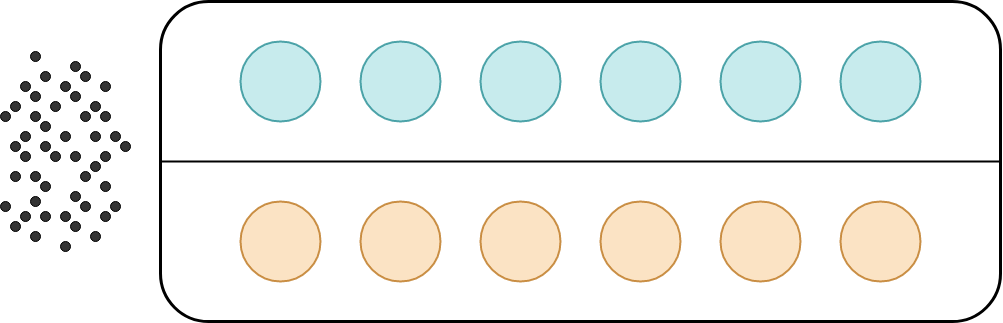
\includegraphics[width=.55\linewidth]{./images/rules-composition.png}
        \caption{Composition du jeu : plateau à $2 \times 6$ trous et 48 graines}
    \end{figure}

    \paragraph{}
    Au début du jeu, 4 graines sont placées dans chaque trou. Les joueurs se trouvent de part et d'autre du plateau, face à leur rangée de graines. Tour à tour, chacun va semer ses graines et tenter d'en récolter. 
    
    \paragraph{}
    A chaque tour, le joueur saisit les graines se trouvant dans l'un de ses trous et les sème une par une dans les trous suivants (dans le sens antihoraire), y compris dans ceux de son adversaire et à l'exception du trou de départ (s'il sème plus de 11 graines, il devra sauter le trou de départ et continuer à partir du suivant).

    \begin{figure}[H]
        \centering
        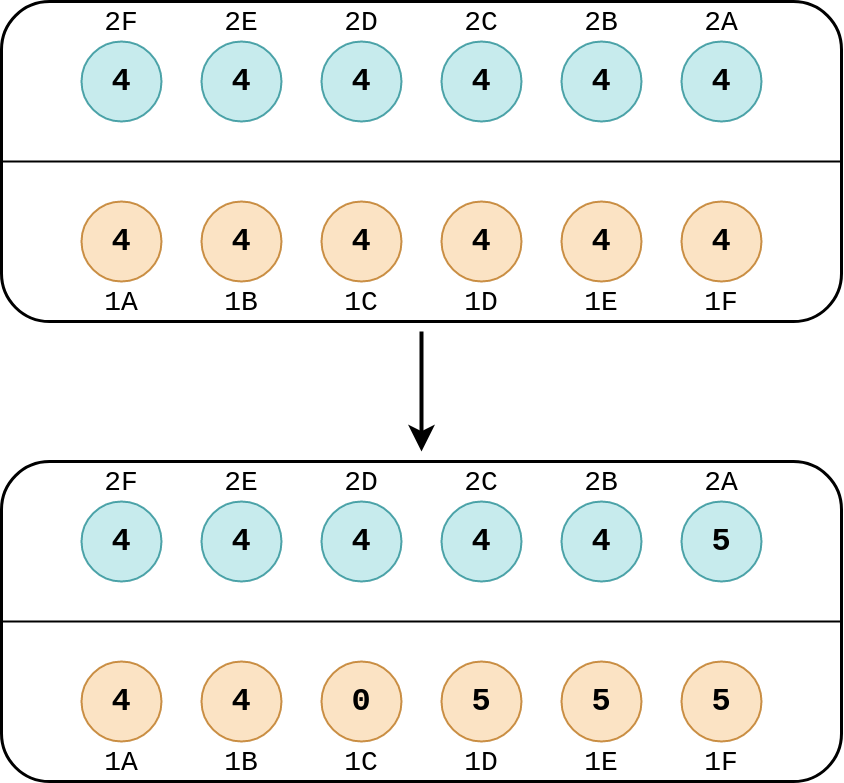
\includegraphics[width=.55\linewidth]{./images/tour1.png}
        \caption{Premier tour : le joueur 1 sème les graines de la case C}
    \end{figure}

    \paragraph{}
    Si la dernière graine est semée dans un des trous adverses et que ce dernier comptait 1 ou 2 graines avant le semis, le joueur prend le contenu de ce trou. Si le trou précédent compte lui aussi 2 ou trois graines après le semis, le joueur peut également les récolter et ainsi de suite. La récolte s'arrête dès que le joueur tombe sur un trou qui compte plus de 3 graines ou s'il revient à la première case adverse.

    \begin{figure}[H]
        \centering
        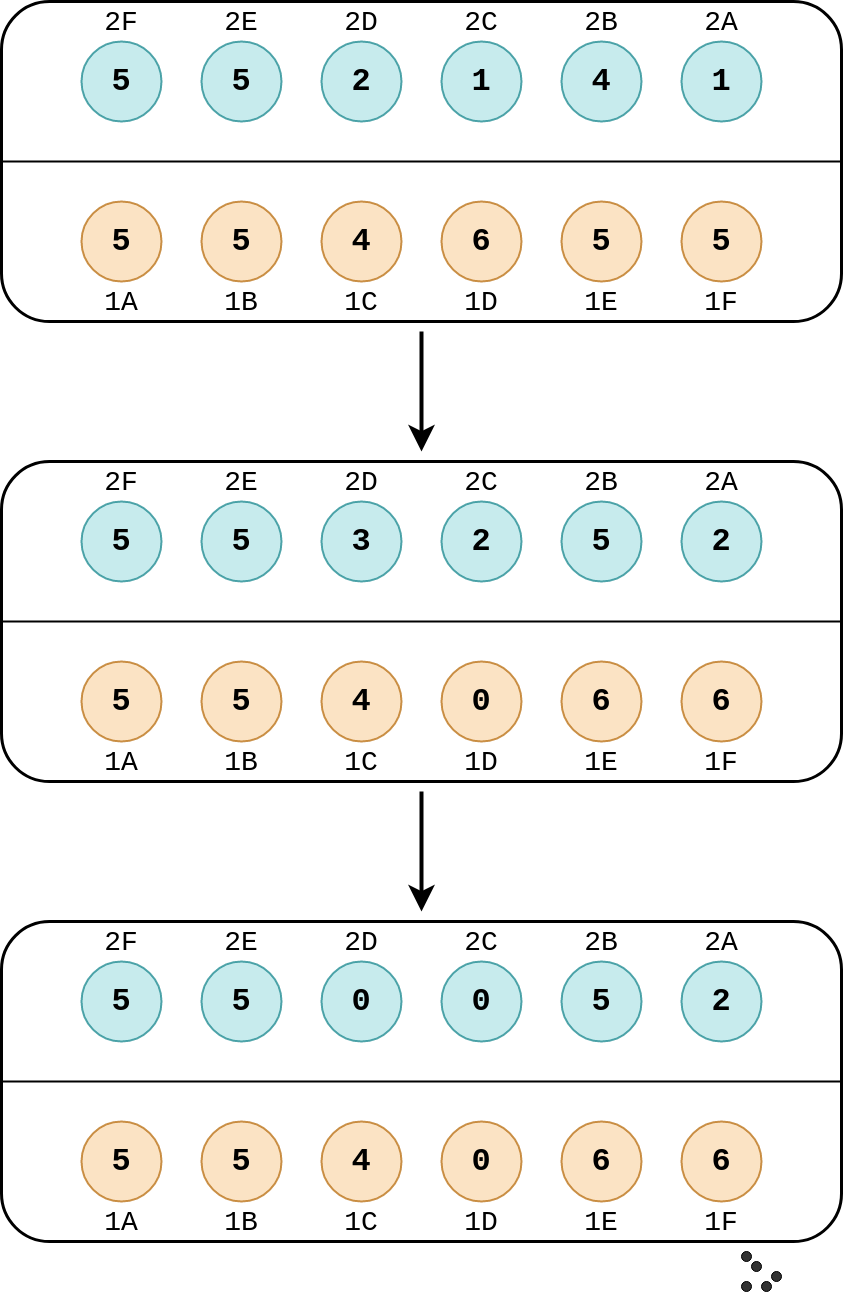
\includegraphics[width=.55\linewidth]{./images/recolte1.png}
        \caption{Le joueur 1 sème les graines de la case D et récolte 5 graines}
    \end{figure}
    
    \paragraph{}
    Il est obligatoire de nourrir l'adversaire : si un des joueurs se retrouve sans graines, l'autre doit à son tour semer des graines dans les cases adverses.

    \paragraph{}
    Il est interdit d'affamer l'adversaire : la rangée d'un joueur ne peut pas être entièrement récoltée par son adversaire. Si un semis entraîne une récolte qui affame l'adversaire, cette récolte ne peut pas se faire.

    \paragraph{}
    La partie peut s'arrêter dès que l'un des deux joueurs a récolté plus de 24 graines mais elle peut aussi continuer pour compter les points.
    
    \paragraph{}
    La partie s'arrête obligatoirement dès qu'il est impossible pour un des joueurs de nourrir l'adversaire affamé : ce joueur peut alors récolter les graines qui se trouvent encore sur sa rangée.


    \newpage
    \section{Diagramme de cas d'utilisation}

    \paragraph{}
    \begin{itemize}
        \item jouer une partie
        \item choisir la difficulté
        \item consulter les scores
        \item enregistrer un score
    \end{itemize}

    \newpage
    \section{Diagramme de séquence système}
    
    \paragraph{}
    Diagramme de séquence global qui reprend les références aux diagrammes de séquences développés plus loi : utilisateur joue et machine joue.


    \begin{itemize}
        \item Consulter les scores
        \item Démarrer une partie : nom du joueur ? Difficulté ?
        \item Boucle principale : joueur 1 joue puis joueur 2 joue
        \item Jusqu'à alt -> joueur 1 gagne / joueur 2 gagne / impossible de continuer
        \item opt enregistrer le score
        \item -> le joueur arrête la partie en cours (entre "quitter" au lieu d'entrer le numéro du trou à jouer)
    \end{itemize}
    Note : c'est toujours le joueur 1 (personne) qui commence à jouer


    \newpage
    \section{Diagramme de classes d'analyse}

    \paragraph{}
    Uniquement les classes nécessaires à la logique du jeu -> diagramme plus détaillé (MVC, etc) = classes de conception

    \begin{itemize}
        \item Partie (singleton, contrôleur) : 1 plateau, 40 graines, 2 joueurs, bool terminé/en cours
        \item Plateau : 8 trous
        \item Trou : appartient à un joueur, nb graines, prendre les graines, ajouter une graine
        \item Joueur virtuel : Joueur aléatoire ou joueur intelligent (héritage)
        \item 
    \end{itemize}


    \newpage
    \section{Diagramme d'états}

    \paragraph{}
    nécessaire ? pour quoi ?


    \newpage
    \section{Séquence : joueur joue}

    \paragraph{}
    Entre un nombre (vérif si pas vide, puis vérif si obligation de nourrir) -> partie -> plateau -> case -> répartition sur les autres cases
    Dernière case : case adverse ? nombre de graines ? -> récolter ou non -> case précédente, etc jusqu'à case 1 adversaire
    Si récolte : mise à jour du score (réserve)

    \newpage
    \section{Séquence : machine joue}

    \paragraph{}
    Idem sauf pour le choix du nombre


    \newpage
    \paragraph{Diagramme de classes de conception}

    \paragraph{}
    Classes détaillées avec champs et méthode (et design patterns).

    \paragraph{}
    Packages MVC
    Vue : classe qui affiche en console / récupère les données utilisateur -> passe à la partie (contrôleur)



    
    
    




    \section*{Conclusion}
    \label{sec:concl}
    \addcontentsline{toc}{section}{\nameref{sec:concl}}


\end{document}